\chapter{Literature Review}
\label{cha:literature-review}

Understanding how developers use language features
and \api{}s is a broad topic.
There is plenty of research in the computer science literature about
empirical studies of programs which involves multiple \emph{dimensions}
directly related to our plan.
Over the last decades,
researchers always have been interested in understanding what
kind of programs developers write.

The importance of conducting empirical studies of programs gave rise to the International Conference on Mining Software Repositories%
\footnote{\url{http://www.msrconf.org/}}
in 2004.

\section*{Outline}

When conducting empirical studies about programs,
multiple dimensions are involved.
The first one is \emph{What to analyse?}
Benchmarks and corpora are used as a source of programs to analyse.
Another aspect is how to select good candidate projects from a large-base software repository.
This is presented in Section~\ref{sec:literature-review:benchmarks}.
After the selection of programs to analyse is set,
comes the question \emph{how to analyse them?}
An overview of what tools are available to extract information from software repositories is given in Section~\ref{sec:literature-review:mining}.
With this infrastructure, \emph{what questions do researchers ask?}
In Section~\ref{sec:literature-review:largescale},
we give an overview of large-scale empirical studies that show what kind of questions researchers ask.
In particular, this section ends by presenting the related work more specific to the Unsafe API and Casting in Sections~\ref{sec:literature-review:unsafe} and \ref{sec:literature-review:casting} respectively.
Finally, Section~\ref{sec:literature-review:conclusions} concludes this chapter.

\section{Benchmarks and Corpora}
\label{sec:literature-review:benchmarks}

Benchmarks are crucial to properly evaluate and measure product development.
This is key for both research and industry.
One popular benchmark suite for \java{} is the DaCapo Benchmark~\citep{blackburnDaCapoBenchmarksJava2006}.
This suite has been already cited in more than thousand publications, showing how important is to have reliable benchmark suites.
The SPECjvm2008\footnote{\url{https://www.spec.org/jvm2008/}}
(Java Virtual Machine Benchmark)
and
SPECjbb2000\footnote{\url{https://www.spec.org/jbb2000/}}
(Java Business Benchmark)
are another popular \java{} benchmark suite.

Another suite has been developed by~\cite{temperoQualitasCorpusCurated2010}.
They provide the Qualitas Corpus, a corpus of curated open source systems to facilitate empirical studies on source code.
On top of the Qualitas Corpus,~\cite{dietrichXCorpusExecutableCorpus2017} provide an executable corpus of \java{} programs.
This allows any researcher to experiment with both static and dynamic analysis.

For any benchmark or corpus to be useful and reliable,
it must faithfully represent real-world code.
For instance,
DaCapo applications were selected to be diverse real applications and
ease of use, but they ``excluded GUI applications since they are difficult
to benchmark systematically.''
Along these lines, \cite{allamanisMiningSourceCode2013} go one step further and provide a large-scale (14,807) curated corpus of open source \java{} projects.

With the advent of cloud computing,
several source code management (SCM) hosting services have emerged, \eg{},
\github{}, \gitlab{}, \bitbucket{}, and \sourceforge{}.
These services allow the developer to work with different SCMs, \eg,
Git, Mercurial, Subversion to host their open source projects.
These projects are usually taken as a representation of
real-world applications.
Thus, while not curated corpora, these hosting services are
commonly used to conduct empirical studies.

Another dimension to consider when analysing large codebases, is how relevant the repositories are.
\cite{lopesDeJaVuMapCode2017} conducted a study to measure code duplication in \github{}.
They found out that much of the code there is actually duplicated.
This raises a flag when considering which projects to analyse when mining software repositories.

\cite{baxterCloneDetectionUsing1998} propose a clone detection algorithm using Abstract Syntax Trees,
while \cite{riegerVisualDetectionDuplicated} propose a visual detection for clones.
\cite{yuanCMCDCountMatrix2011,chenReplicationReproductionCode} instead propose Count Matrix-based approach to detect code clones.

\cite{nagappanDiversitySoftwareEngineering2013} have developed the Software Projects Sampling (SPS) tool.
SPS tries to find a maximal set of projects based on representativeness and diversity.
Diversity dimensions considered include total lines of code,
project age, activity, number of contributors, total code churn,
and number of commits.

\section{Tools for Mining Software Repositories}
\label{sec:literature-review:mining}

When talking about mining software repositories,
we refer to extracting any kind of information from large-scale codebase repositories. 
Usually doing so requires several engineering but challenging tasks.
The most common being downloading, storing, parsing, analysing and
properly extracting information from different kinds of artifacts.
In this scenario, there are several tools that allows a researcher or developer to query information about software repositories.

\cite{urmaProgrammingLanguageEvolution2012} evaluated seven source code
query languages:
\emph{Java Tools Language}~\citep{cohenJTLJavaTools},
\emph{SOUL}~\citep{derooverSOULToolSuite2011},
\emph{Browse-By-Query}\footnote{\url{http://browsebyquery.sourceforge.net/}},
\emph{JQuery}~\citep{volderJqueryGenericCode2006},
\emph{.QL}~\citep{moorKeynoteAddressQL2007},
\emph{Jackpot}\footnote{\url{http://wiki.netbeans.org/Jackpot}}, and
\emph{PMD}\footnote{\url{https://pmd.github.io/}}.
They have implemented, whenever possible,
four use cases using the tools mentioned above.
They concluded that only \emph{SOUL} and \emph{.QL} have the minimal features to implement all their use cases.

\cite{dyerBoaLanguageInfrastructure2013,dyerDeclarativeVisitorsEase2013} built \boa{}, both a domain-specific language and an online platform\footnote{\url{http://boa.cs.iastate.edu/}}. 
It is used to query software repositories on two popular hosting services, \github{} and \sourceforge{}.
The same authors of \boa{} conducted a study on
how new \java{} features, \eg,
\emph{Assertions},
\emph{Enhanced-For Loop},
\emph{Extends Wildcard},
were adopted by developers over time~\citep{dyerMiningBillionsAST2014}.
This study is based \sourceforge{} data.
The current problem with \sourceforge{} is that is outdated.

To this end, \cite{gousiosGHTorentDatasetTool2013} provides an offline mirror of \github{} that allows researchers to query any kind of that data.
Later on, \cite{gousiosLeanGHTorrentGitHub2014} published the dataset construction process of \github{}.

Similar to \boa{}, \lgtm{}\footnote{\url{https://lgtm.com/}} is a platform to query software projects properties.
It works by querying repositories from \github{}.
But it does not work at a large-scale, \ie{}, \lgtm{} allows the user to query just a few projects.
Unlike \boa{}, \lgtm{} is based on \ql{}---before named \emph{.QL}---,
an object-oriented domain-specific language to query recursive data structures based on Datalog~\citep{avgustinovQLObjectorientedQueries2016}.
Another static analysis framework based on Datalog is \doop{}~\citep{bravenboerStrictlyDeclarativeSpecification}.
Since \ql{} and \doop{} are based on Datalog,
both are well-suited to perform points-to analysis and data-flow analysis.
However, scaling such analysis to a large-scale study remains an open problem.

On top of \boa{},~\cite{tiwariCandoiaPlatformBuilding2017} built \candoia{}%
\footnote{\url{http://candoia.github.io/}}.
Although it is not a mining software repository \perse{},
it eases the creation of mining applications. 

Another tool to analyse large software repositories is presented in~\cite{brandauerSpencerInteractiveHeap2017}.
In this case, the analysis is dynamic, based on program traces. 
At the time of this writing, the service\footnote{\url{http://www.spencer-t.racing/datasets}} was unavailable for testing. 

\cite{bajracharyaSourcererInternetscaleSoftware2009} provide a tool to query large code bases by extracting the source code into a relational model.
Sourcegraph\footnote{\url{https://sourcegraph.com}} is a tool that allows regular expression and diff searches.
It integrates with source repositories to ease navigate software projects.

\cite{posnettTHEXMiningMetapatterns2010} have extended
\asm{}~\citep{brunetonASMCodeManipulation2002}
to detect meta-patterns, \ie{},
structural patterns of object-oriented interaction.
\cite{huDynamicAnalysisDesign2008} used both dynamic and static analysis to discover design patterns, while \cite{arcelliDesignPatternDetection2008} used only dynamic analysis.

Trying to unify analysis and transformation tools,
\cite{vinjuHowMakeBridge2006} and~\cite{klintRASCALDomainSpecific2009} built \rascal{},
a DSL that aims to bring them together by querying the AST of a program.
Spoon is a \java{} library
``to analyse, rewrite, transform, transpile \java{} source code''~\citep{pawlak:hal-01169705}.
It supports symbol resolution natively and match code elements using Spoon patterns.
Probably one of the most mature libraries to parse and manipulate \java{} source code is Eclipse \java{} Development Tools (JDT).%
\urlnote{https://www.eclipse.org/jdt/}
Besides parsing \java{} source code,
Eclipse JDT has the ability to compile, run, and debug \java{} source code.
ExtendJ~\citep{Ekman:2007:JEJ:1297027.1297029} is an extensible \java{} compiler.
It supports semantic analysis and bytecode generation.
With \java{} 8, it is possible to write plug-ins for the \javac{} compiler.
By writing a compiler plug-in, it is possible to add extra-compile checks,
perform code transformations and custom analysis.
JavaParser,\footnote{\url{http://javaparser.org/}} as its name suggests,
is a parser for \java{}.
The main issue with JavaParser is that it lacks the ability to perform symbol resolution integrated with project dependencies.
javalang\urlnote{https://github.com/c2nes/javalang} is a library written in \python{} to parse \java{} source code.

In early prototypes of our cast study we have used
javalang and a custom \javac{} plug-in,%
\urlnote{https://gitlab.com/acuarica/java-cast-inspection}
and JavaParser%
\urlnote{https://gitlab.com/acuarica/java-cast-study}
to parse and analyse \java{} source code.


\section{Empirical Studies of Large Codebases}
\label{sec:literature-review:largescale}

In the same direction as our plan,
\cite{callauHowWhyDevelopers2013} performed an empirical study to assess
how much the dynamic and reflective features of \smalltalk{} are actually
used in practice.
Analogously, \cite{richardsAnalysisDynamicBehavior2010,richardsEvalThatMen2011,weiEmpiricalStudyDynamic2016}
conducted a similar study, but in this case targeting \javascript's dynamic
behavior and in particular the \code{eval} function.
Also, for \javascript{}, \cite{madsenStringAnalysisDynamic2014} analysed
how fields are accessed via strings,
while~\cite{jangEmpiricalStudyPrivacyviolating2010}
analysed privacy violations.
Similar empirical studies were done for
\php{}~\citep{hillsEmpiricalStudyPHP2013,dahseExperienceReportEmpirical2015,doyleEmpiricalStudyEvolution2011}
and \swift{}~\citep{reboucasEmpiricalStudyUsage2016}.
\cite{PINTO201559} conducted a large-scale study on how concurrency is used in \java{}

Going one step forward, \cite{rayLargescaleStudyProgramming2017} studied the correlation between programming languages and defects. 
One important note is that they choose relevant projects by popularity,
measured by how many times the project was \emph{starred} in \github{}.

\cite{gorlaCheckingAppBehavior2014} mined a large set of Android applications, clustering applications by their description topics and identifying outliers in each cluster with respect to their API usage.
\cite{grechanikEmpiricalInvestigationLargescale2010} also mined large scale software repositories to obtain several statistics on how source code is actually written.

For \java{},~\cite{dietrichContractsWildStudy2017a} conducted a study
about how programmers use contracts in \mavencentral{}\footnote{\url{http://central.sonatype.org/}}.
\cite{dietrichBrokenPromisesEmpirical2014} have studied how
\api{} changes impact \java{} programs.
They have used the Qualitas Corpus~\citep{temperoQualitasCorpusCurated2010} mentioned above for their study.

\cite{tufanoWhenWhyYour2015,tufanoWhenWhyYour2017} studied when code
smells are introduced in source code.
\cite{palombaLandfillOpenDataset2015}
contribute a dataset of five types of code smells together with a systematic procedure for validating code smell datasets.
\cite{palombaDetectingBadSmells2013} propose to detect code smells using change history information.

\cite{nagappanEmpiricalStudyGoto2015} conducted a study on how the
\code{goto} statement is used in \cc{}.
They used \github{} as a data source for \cc{} programs.
They concluded that \code{goto} statements are most used for
\emph{handling errors} and \emph{cleaning up resources}.

\textbf{Static vs. Dynamic Analysis.}
Given the dynamic nature of \javascript, most of the studies mentioned
above for \javascript{} perform dynamic analysis.
However, \cite{callauHowWhyDevelopers2013} uses static analysis to study
a dynamically checked language.
For \java{}, most empirical studies use static analysis.
This is due to the unavailability of input data.
Finding valid input data for test cases is not a trivial task.
For \javascript{}, having a big corpus of web-sites generating valid
input data makes more feasible to implement dynamic analysis.

\subsection*{Programming Language Features}

Programming language design has been always a hot topic in computer science literature.
It has been extensively studied in the past decades.
There is a trend in incorporating programming features into mainstream object-oriented languages, \eg,
lambdas in \java{} 8\footnote{\url{https://docs.oracle.com/javase/specs/jls/se8/html/jls-15.html\#jls-15.27}},
\cpp{}11\footnote{\url{http://www.open-std.org/jtc1/sc22/wg21/docs/papers/2006/n1968.pdf}} and
\csharp{} 3.0\footnote{\url{https://msdn.microsoft.com/en-us/library/bb308966.aspx\#csharp3.0overview\_topic7}};
or parametric polymorphism, \ie{}, generics, in \java{} 5.%
\urlnote{https://docs.oracle.com/javase/1.5.0/docs/guide/language/generics.html}%
\(^{,}\)%
\urlnote{http://www.oracle.com/technetwork/java/javase/generics-tutorial-159168.pdf}
For instance, \java{} generics were designed to extend
\java's type system to allow
``a type or method to operate on objects of various types while
providing compile-time type safety''
\citep{Gosling:2013:JLS:2462622}.
However, it was later shown~\citep{aminJavaScalaType2016} that 
compile-time type safety was not fully achieved.

\cite{keryExaminingProgrammerPractices2016,asaduzzamanHowDevelopersUse2016} focus on exceptions.
They conducted empirical studies on how programmers handle exceptions in \java{} code.
The work done by~\cite{nakshatriAnalysisExceptionHandling2016} categorized them into patterns.
\cite{coelhoUnveilingExceptionHandling2015} used a more dynamic approach by analysing stack traces and code issues in \github{}.
\cite{kechagiaUndocumentedUncheckedExceptions2014} analysed how undocumented and
unchecked exceptions cause most of the exceptions in
Android applications.

\cite{mazinanianUnderstandingUseLambda2017} and \cite{uesbeckEmpiricalStudyImpact2016} studied how developers use lambdas in \java{} and \cpp{} respectively.
The inclusion of generics in \java{} is closely related to collections. 
\cite{parninJavaGenericsAdoption2011,parninAdoptionUseJava2013} studied how generics were adopted by \java{} developers.
They found that the use of generics does not significantly reduce the number of type casts.

\cite{costaEmpiricalStudyUsage2017} have mined \github{} corpus to study the use and performance of collections,
and how these usages can be improved.
They found that in most cases there is an alternative usage that improves performance.

Another study about how a programming language feature is used is done in
\cite{temperoHowJavaPrograms2008}.
They conducted a study on how inheritance is used in \java{} programs.

This kind of studies give an insight of the adoption of lambdas and generics, which can drive future direction for language designers and tool builders, while providing developers with best practices.

\subsection{Unsafe Intrinsics in \java{}}
\label{sec:literature-review:unsafe}

Oracle provides the \smu{} class for low-level programming,
\eg{}, synchronization primitives, direct memory access methods,
array manipulation and memory usage.
Although \smu{} is not officially documented,
it is being used in both industrial applications
and research projects~\citep{korlandNoninvasiveConcurrencyJava2010,pukallFlexibleDynamicSoftware,gligoricCoDeSeFastDeserialization2011}
outside the JDK, compromising the safety of the \java{} ecosystem.

Oracle's software engineer Paul Sandoz performed an informal analysis of
\mavencentral{} artifacts and usages in Grepcode~\citep{sandoz-personal-communication}
and conducted a unscientific user survey to study how the \unsafe{} \api{} is used~\citep{psandoz14}.
The survey consists of 7 questions,%
\urlnote{http://www.infoq.com/news/2014/02/Unsafe-Survey}%
\(^{,}\)%
\urlnote{http://cr.openjdk.java.net/~psandoz/dv14-uk-paul-sandoz-unsafe-the-situation.pdf}
that help to understand what pieces of \smu{} should be mainstreamed.
In his survey,
he found out that most developers that use \smu{} \emph{do not} have a fallback when \smu{} is not presence,
thus undermining portability.
Similarly, most developers are willing to replace Unsafe with safer alternatives---new API or language changes---in the case there is one.
Figure~\ref{fig:lr:unsafe4} shows the answers to the question:
\emph{``What reasons did you use Unsafe for?''}
These reasons are somewhat related to our Unsafe usage patterns.
We complement his survey to identify more use cases of Unsafe in a large codebase.
When studying a larger codebase some results might change.
For instance, he concluded that the \code{monitorEnter/monitorExit/tryMonitorEnter} methods are not used,
whereas in our study we found out (see Section \ref{sec:unsafe:overview:features})that only \code{tryMonitorEnter} is never used.

\begin{figure}[ht!]
\centering
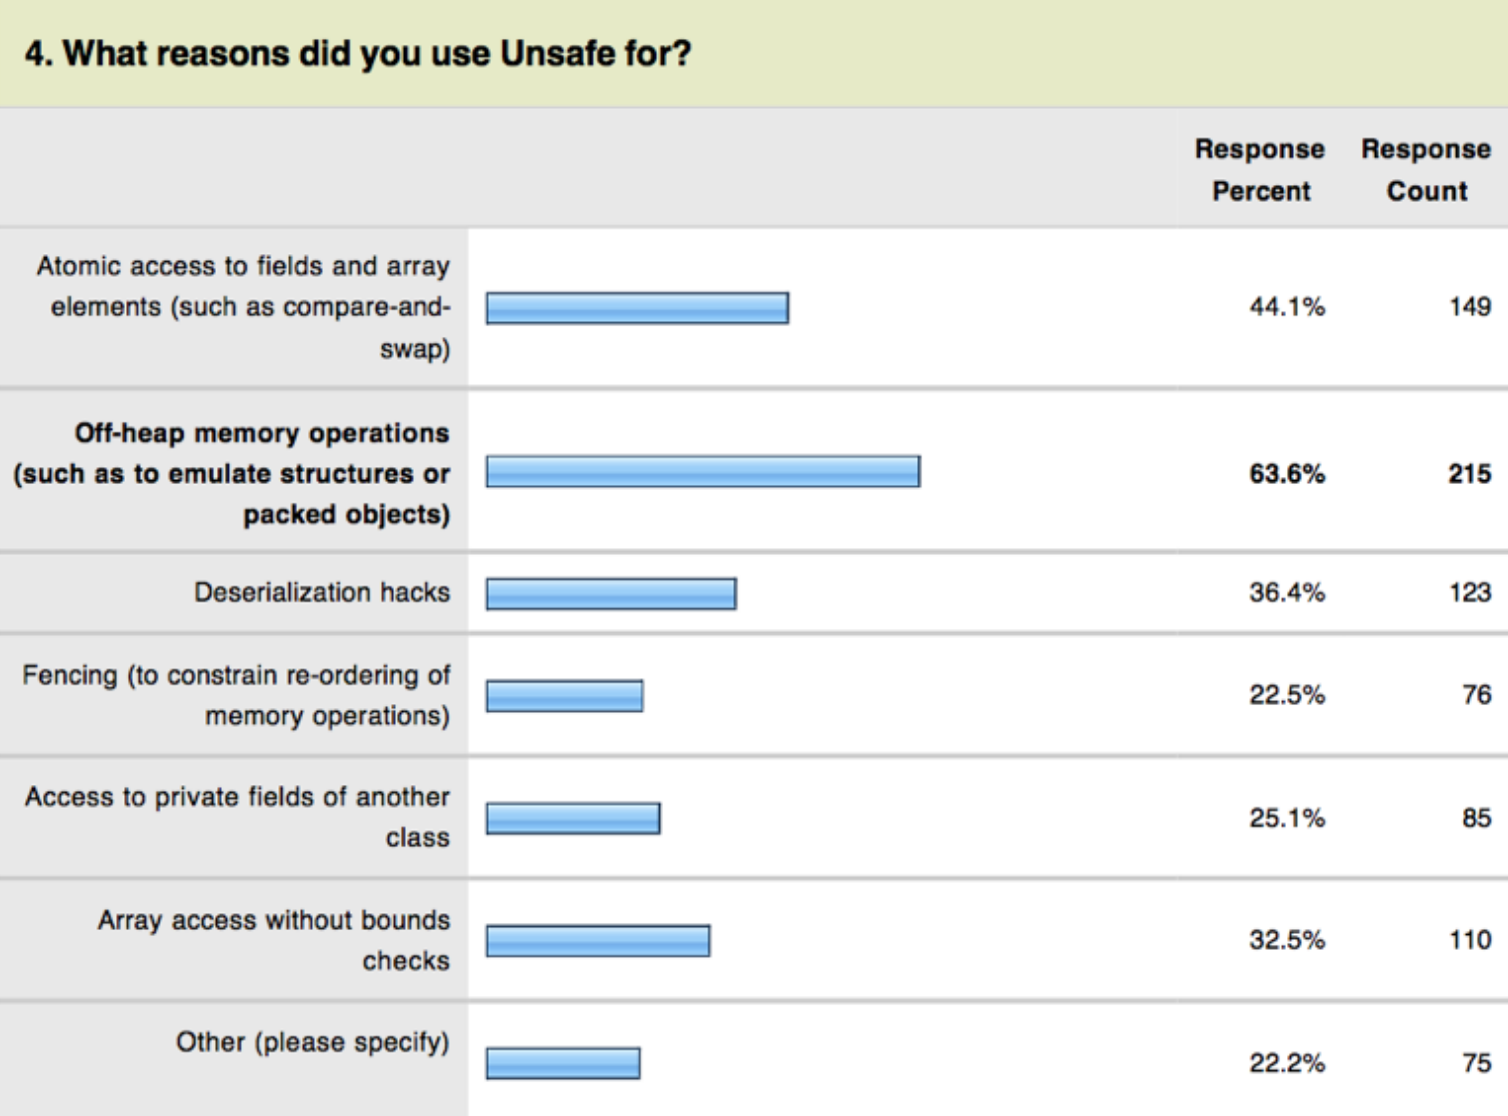
\includegraphics[width=\textwidth]{Unsafe-Survey-4}
\caption{Categorization of Unsafe usages from Sandoz' survey} \label{fig:lr:unsafe4}
\end{figure}

\cite{tanSafeJavaNative2006} propose a combination of static and dynamic checks to provide a safe variant of the \java{} Native Interface (\jni{}).
They have identified several loopholes that may cause unsafe interoperation between \java{} and native code.
The language extension provided by~\cite{Bubak00creatingjava}
allows the developer to interleave \java{} and native code in the same compilation unit.
However, the native code is not---statically nor dynamically---checked,
causing a possible \jvm{} crash.
\cite{tanEmpiricalSecurityStudy2008} and~\cite{kondohFindingBugsJava2008}
conducted an empirical security study to describe a taxonomy to classify bugs when using \jni{}.
\cite{sunNativeGuardProtectingAndroid2014} develop a method to isolate native components in Android applications.
\cite{liFindingBugsExceptional2009} analyse the discrepancy between how exceptions are handled in native code and \java{}.

\subsection{Reflective Capabilities}
\label{sec:literature-review:casting}

\cite{livshitsImprovingSoftwareSecurity2006,livshitsReflectionAnalysisJava2005} ``describes an approach to call graph construction for \java{} programs in the presence of reflection.''
He has devised some common usage patterns for reflection.
More precisely, he identified 7 reflection usage patterns.
Most of the patterns need a cast operation to actually be able to use some value obtained by reflection.
For instance,
the ``Specifying Application Extensions'' pattern is used to implement a plugin system,
\ie, where classes are dynamically loaded from a configuration file to extend the functionality of a base application.
Usually the class being dynamically loaded needs to implement or extend a specific interface or class respectively to be used by the plugin system.
Thus, a cast is needed to \emph{dynamically} assert that indeed this is the case.
In out study, we plan to categorize all cast usages, not only where reflection is used.

\cite{landmanChallengesStaticAnalysis2017} have analysed the relevance of
static analysis tools with respect to reflection.
They conducted an empirical study to check how often the reflection
\api{} is used in real-world code.
They have devised reflection AST patterns,
which often involve the use of casts.
Finally, they argue that controlled programming experiments on
subjects need to be correlated with real-world use cases,
\eg, \github{} or \mavencentral{}.

Casting operations in \java{}%
\footnote{\url{https://docs.oracle.com/javase/specs/jls/se8/html/jls-15.html\#jls-15.16}}
allows the developer to view a reference at a different type as it was declared.
The related \code{instanceof} operator%
\footnote{\url{https://docs.oracle.com/javase/specs/jls/se8/html/jls-15.html\#jls-15.20.2}}---written \code{e instanceof T}---tests whether a reference \code{e} could be cast to a different type \code{T} without
throwing \code{ClassCastException} at run time.

\cite{wintherGuardedTypePromotion2011} has implemented a
path sensitive analysis that allows the developer to avoid casting
once a guarded \code{instanceof} is provided.
He proposes four cast categorizations according to their
run-time type safety:
\emph{Guarded Casts}, \emph{Semi-Guarded Casts},
\emph{Unguarded Casts}, and \emph{Safe Casts}.

\cite{tsantalisJDeodorantIdentificationRemoval2008} present an
Eclipse plug-in that identifies type-checking bad smells,
a ``variation of an algorithm that should be executed,
depending on the value of an attribute''.
They provide refactoring analysis to remove the detected smells
by introducing inheritance and polymorphism.
This refactoring will introduce casts to select
the right type of the object.

\textbf{Controlled Experiments on Subjects.}
There is an extensive literature \perse{} in controlled experiments on subjects to understand several aspects in programming, and programming languages.
For instance,~\cite{solowayEmpiricalStudiesProgramming1984} tried to understand how expert programmers face problem solving.
\cite{buddTheoreticalEmpiricalStudies1980} conducted an empirical study on how effective mutation testing is.
\cite{precheltEmpiricalComparisonSeven2000} compared how a given---fixed---task was implemented in several programming languages.
\cite{latozaDevelopersAskReachability2010} realize that, in essence, programmers need to answer reachability questions to understand large codebases.
Several authors~\cite{stuchlikStaticVsDynamic2011,mayerEmpiricalStudyInfluence2012,harlinImpactUsingStaticType2017} measure whether using a static-type system improves programmers productivity.
They compare how a static and a dynamic type system impact on productivity.
The common setting for these studies is to have a set of programming problems.
Then, let a group of developers solve them in both a static and dynamic languages.
For this kind of studies to reflect reality, the problems to be solved need to be representative of the real-world code.
Having artificial problems may lead to invalid conclusions.
The work by~\cite{wuHowTypeErrors2017,wuLearningUserFriendly2017} goes towards this direction. 
They have examined programs written by students to understand real debugging conditions. 
Their focus is on ill-typed programs written in \haskell{}.

\section{Conclusions}
\label{sec:literature-review:conclusions}

The \java{} Native Interface and \java{}'s reflection \api{} are well-studied topics.
Several studies have been conducted to understand why developers use these features,
and several analyses have been devised to check whether their usage is correct.

But \java{}'s unsafe intrinsics and reflection capabilities comprise more than \jni{} and reflection \api{}.
Unsafe operations can be performed by using the undocumented \smu{} class.
The cast operator provides a lightweight form of type introspection.
However---to our knowledge---these features have never been studied before in the literature.
Moreover,
given that the cast operator is part of the \java{} language itself,
we believe its use is more widespread than the reflection \api{}.
This thesis provides the first empirical studies on the \unsafe{} \api{} and cast operator in \java{}.
In our work~\citep{mastrangeloUseYourOwn2015} we extend Sandoz' work
by performing a comprehensive study of the \mavencentral{}
software repository to analyse how and when \smu{} is being used.
This study is summarized in Chapter~\ref{cha:unsafe}.
We refined the categorization performed by \cite{wintherGuardedTypePromotion2011} to answer our~\ref{casts:rq2} (\emph{\crqB}).
This is described in Chapter~\ref{cha:casts}.
We believe that understanding how and when developers use these features can provide informed decisions for the future of \java{} while providing a guide for developers with better or best practices.
